% 第三篇CellCharter毕业论文第四章结果与分析：2026-11-22首版重写
% 本稿为论文写作草稿，待导师确认章节编号、全论文术语、图件排版。
% 证据入口：RESULTS_ARCHIVE_STATUS_20261122.md
% 不改写任何实验数据；2026-11-22后的E3d后验ARI/NMI及E3b容差均为明确标记的post-hoc分析。
% 警告：如在主文件中用\chapter{...}引入本稿，请调整本文件首行section层级。
\section{实验结果与分析}
\label{sec:cellcharter-results-v1}

\subsection{评价任务、数据结构与报告口径}
\label{subsec:cellcharter-design-v1}

本章围绕空间转录组聚类结果的三个问题开展实证分析：多尺度邻域表征的深度是否影响空间域划分，无标签聚类数选择是否改变性能评价，以及聚类质量与空间边界定位之间是否存在不同的变化趋势。在此基础上，本章加入成熟聚类方法对照和独立组织队列评价，以检验相关观察在不同样本中的适用范围。研究使用CellCharter已实现的多尺度邻域特征聚合与聚类流程，对已有表征进行固定组合、累计深度和聚类数设置比较；不将特征重组表述为新提出的基础聚类算法。

主要DLPFC数据包含12张Visium切片，分别来自3位供体，每位供体4张切片。以切片为单位计算聚类评价，以供体作为独立生物学来源；同一供体的4张切片与同一切片的不同技术种子不能视为独立生物学重复。外部评价采用6例乳腺癌患者对应的Visium数据；其中6名患者是独立生物学样本。各分析的均值均明确注明其汇总层级，不对切片、spot、空间边或随机种子实施伪独立统计推断。

聚类结构评价使用调整兰德指数（adjusted Rand index，ARI）和归一化互信息（normalized mutual information，NMI）。其中NMI为算术平均归一化形式。仅在人工参考标注可用的spot上计算两项指标。空间边界评价使用Visium阵列坐标所定义的六邻接无向边，仅保留两个端点均有有效参考标签的边；参考边界定义为相邻spot属于不同参考层，预测边界定义为相邻spot被分入不同原始聚类编号。严格边界F1由真正例TP、假正例FP与假负例FN计算：
\begin{equation}
F_{1,\mathrm{strict}}=\frac{2TP}{2TP+FP+FN}.
\label{eq:cellcharter-boundary-v1}
\end{equation}
严格指标要求预测边界与参考边界在同一图边上完全一致。后验敏感性分析另行考察1-hop、2-hop容差：在有效无向边构成的线图中，以边到边距离定义容差，并以一对一最大基数匹配防止重复将多个预测边界计为同一真实边界的TP。容差F1反映邻近检出，而非严格的边界定位精度，三种结果必须分别报告。

本章区分两种聚类数策略。Oracle-K使用人工参考层的类别数决定K，属于标签类别数知情的评价条件，不等同于无标签模型选择；K-blind不使用参考标签决定聚类数，其标签仅用于预测文件冻结后的后验评分。本研究不将Oracle-K自动视为所有指标的理论上界，也不将不同K选择方式产生的结果混为一组。DLPFC早期开发切片、补充分析及新增的外部队列之间的关系依各阶段原冻结协议解释；本章所有新增后验分析均保留其发生于原模型训练完成之后的时间顺序。

\subsection{多尺度邻域特征与固定K条件下的聚类表现}
\label{subsec:cellcharter-e1e2-v1}
% 数据来源：E1E2_20261119_RELEASE/derived/all_120_condition_stats.csv
% 以及E1E2_20261119_RELEASE/derived/B_vs_A_12slices.csv

首先，在DLPFC的12张切片上，使用10种事先固定的多尺度特征配置和10个技术随机种子完成1200项GMM聚类评价。累计特征配置从$L_0$（5维）逐步增加至$L_0$--$L_4$（25维），另包括若干固定15维的非连续邻域块组合。本阶段的聚类数依据参考标注类别数设定，因此属于Oracle-K条件，评价的是固定K下的特征组织方式差异，而不是自动选K能力。

将每张切片的10个种子先求平均，再对12张切片作等权描述性平均，累计5D、10D、15D、20D、25D配置的ARI依次为0.3051、0.4081、0.4299、0.4383和0.4418；对应NMI为0.4133、0.5422、0.5780、0.5891和0.5982（表\ref{tab:cellcharter-e1e2-depth-v1}）。在这一固定评价条件下，累计深度提高伴随宏平均ARI、NMI上升，但后期增量明显小于由5D增加至10D的初始差值。由于增加邻域层同时提高了输入维度，这些变化不能单独归因于邻域传播范围，也不能证明更深聚合在所有样本上都优越。

\begin{table}[htbp]
\centering
\caption{DLPFC固定Oracle-K下累计邻域特征的聚类表现（12张切片描述性等权均值；每切片先汇总10个技术种子）}
\label{tab:cellcharter-e1e2-depth-v1}
\begin{tabular}{lccc}
\toprule
累计邻域特征 & 维度 & ARI & NMI\\
\midrule
$L_0$ & 5 & 0.3051 & 0.4133\\
$L_0+L_1$ & 10 & 0.4081 & 0.5422\\
$L_0+L_1+L_2$（A） & 15 & 0.4299 & 0.5780\\
$L_0+\cdots+L_3$ & 20 & 0.4383 & 0.5891\\
$L_0+\cdots+L_4$ & 25 & 0.4418 & 0.5982\\
\bottomrule
\end{tabular}
\end{table}

进一步比较维度相同但邻域组合不同的A（$L_0+L_1+L_2$）与B（$L_0+L_1+L_4$），10技术种子汇总后，B相对A的12切片ARI平均变化约为$+0.0033$，NMI平均变化约为$+0.0109$。虽然均值略为正向，其幅度较小，不同供体和切片的变化方向并不一致。早期单个种子下曾观察到B的平均ARI与边界F1下降，说明单次开发性对比不足以推断候选B具有稳定优势。本研究因而保留两种15维配置的全量正负结果，不以个别样本或最优种子取代完整评价。B只是已有特征块的等维重组，而非经过证实的新聚类模型。

\subsection{固定K网格敏感性与无标签AutoK选择}
\label{subsec:cellcharter-e3c-e3d-v1}
% E3c来源：E3C_20261120_RELEASE/e3c_macro_K_depth_20groups.csv
% E3d来源：E3D_POSTHOC_20261122_RELEASE/derived/four_scale_descriptives.csv

为区分邻域表征和聚类数设置的影响，E3c在12张DLPFC切片的10D、15D、20D、25D特征上考察固定$K=5,6,7,8,9$的评价网格。该阶段形成2400个有效条件评价格，其中1920项为新增运行，另480项复用此前经审计的Oracle-K结果。固定K网格中的K由分析设计直接指定，并不是在不知参考标签的条件下自动估计得到。

以15维配置为例，当K从5增加到9时，12切片等权平均ARI由0.4440变为0.3561；20维配置对应为0.4461至0.3664。两组对比提示在当前数据和固定模型条件下，ARI对预设K具有较强敏感性。需要注意的是，K=5只与4张切片的参考类别数一致，而其余8张的Oracle-K类别数为7，因此这并不是对全部切片普遍“正确K”的检验。不同K对应的ARI变化应作为网格敏感性证据，而非选择论文中最好表现K的依据。

针对不使用参考标签选择K的问题，E3d对12张切片与4种累计尺度共48个配置执行原生AutoK流程。正式冻结候选区间为$K\in\{2,\ldots,10\}$，每个配置的内部GMM稳定性评估采用5次技术重复，记录选中K、各候选稳定性与完整预测文件。原始48配置审计全部通过；其中K=2出现9次、K=10出现1次，即10/48次选中冻结搜索边界。此类边界选择作为结果保留，并未在观察到标签后重新扩展搜索范围。

在模型与K选择全部完成后，使用原冻结预测和相同人工参考标签单独开展\textbf{事后后验评价}，计算全部48项ARI/NMI，并由列联表计算独立交叉复核。12张切片等权平均结果见表\ref{tab:cellcharter-e3d-v1}。20维配置的平均ARI和NMI分别为0.4311和0.5942，为这四个配置中的最高描述性均值；但25维相对20维并未继续上升，说明增加尺度与改善指标之间并不存在无条件单调关系。

\begin{table}[htbp]
\centering
\caption{E3d K-blind AutoK完成后的事后ARI/NMI评价（12切片等权描述性均值，独立供体$n=3$）}
\label{tab:cellcharter-e3d-v1}
\begin{tabular}{lccc}
\toprule
特征维度 & ARI & NMI & K搜索边界命中数/12\\
\midrule
10D & 0.3793 & 0.5033 & 4\\
15D & 0.3861 & 0.5359 & 2\\
20D & 0.4311 & 0.5942 & 1\\
25D & 0.3890 & 0.5434 & 3\\
\bottomrule
\end{tabular}
\end{table}

例如15D的K-blind均值ARI为0.3861，而E1/E2标签类别数知情Oracle-K、10技术种子的相应切片宏平均ARI约为0.4299，两者不能被简单解释为“无标签化必然带来0.0438的损失”。这两组任务的K规则、初始化和重复结构不同，比较反映的是现有完整工作流程的描述性差异，并不是只替换K策略的受控因果实验。特别是K选择与邻域深度可能共同改变实际簇数，本研究不将20维结果归因为单一聚合机制。

\subsection{空间边界的严格检出与容差敏感性}
\label{subsec:cellcharter-e3b-v1}
% E3b来源：E3B_E1E2_1200_POSTHOC_20261122_RELEASE/derived/macro_mean_30.csv
% E3d Kblind补充：E3B_E3D48_POSTHOC_20261122_RELEASE/

ARI与NMI描述整体参考标签和聚类分配之间的一致性，但两项指标并不要求预测聚类在空间上准确定位层间交界。因此，本研究使用已有冻结预测进一步开展空间边界审查。E3b是在既有实验结果已被观察之后追加的\textbf{事后敏感性评价}，没有改变任何预测聚类或参考标签；在E1/E2完整的1200份Oracle-K预测上，分别计算严格0-hop、1-hop、2-hop三种线图容差，共得到3600条边界评价记录。

表\ref{tab:cellcharter-boundary-v1}列示5种累计尺度的完整主要趋势，每项均为先在相同切片内汇总10技术种子，再对12张切片作等权描述性平均。严格边界F1从5D的0.1441变化至25D的0.1179，总体未随尺度加深而提高；相比之下2-hop容差F1从0.2863增加至0.5333。25D在这5种累计配置中的2-hop均值最高，却具有最低严格F1。该观察表明对“边界是否准确定位”的判断依赖评价空间容差；不能因宽松容差分数较高，就得出精确边界检出更好的结论。

\begin{table}[htbp]
\centering
\caption{E1/E2完整1200预测的边界评价（12切片等权均值；Oracle-K；0/1/2-hop属于事后敏感性分析）}
\label{tab:cellcharter-boundary-v1}
\begin{tabular}{lccc}
\toprule
累计特征 & 严格0-hop F1 & 1-hop F1 & 2-hop F1\\
\midrule
5D & 0.1441 & 0.2621 & 0.2863\\
10D & 0.1446 & 0.3369 & 0.4116\\
15D & 0.1361 & 0.3559 & 0.4838\\
20D & 0.1344 & 0.3614 & 0.5223\\
25D & 0.1179 & 0.3457 & 0.5333\\
\bottomrule
\end{tabular}
\end{table}

这一差异与更深邻域表征可能改变局部预测边界的位置或粗细相容，但目前结果只能证明评价指标之间的权衡，尚不足以单独确立“空间平滑造成边界扩宽”的因果机制，因为邻域层数增加同时改变了输入维度和模型结果。对于另行冻结的E3d K-blind 48份预测，本研究也按同一边界定义完成严格及容差评价；10/15/20/25D的严格F1均值分别为0.1596、0.1299、0.1338、0.1190。两种K设置应独立呈现，不将其合并计算为独立重复。

为校验本次边界计算与历史记录的一致性，对E1/E2的技术种子22911下A15D与B15D进行严格TP计数核对：12切片累计TP分别为2103和1999，与此前独立边界记录完全相符。这一核对支持边定义及基础计数实现的一致性，但并不自动证明所有容差指标具有生物学解释力。

\subsection{与成熟空间聚类方法的对比}
\label{subsec:cellcharter-e5a-v1}
% E5a来源：E5A_20261122_RELEASE/derived/method_regime_descriptives.csv

E5a在同一12张DLPFC切片上引入非空间GMM、Leiden、BANKSY及BayesSpace作为成熟对照。四种基线均保留K-blind和Oracle-K条件，每条件重复3个技术种子，共288项经独立审计的结果。GMM与Leiden使用相同的5维scVI基础特征，BANKSY与BayesSpace使用其原生计数输入及各自的空间处理流程，因此本节属于在明确预处理差异前提下的成熟方法表现比较，而非完全同特征、同计算预算的单变量对照。

\begin{table}[htbp]
\centering
\caption{E5a四种基线在DLPFC上的ARI（12张切片等权均值，独立供体$n=3$；不同K条件分开）}
\label{tab:cellcharter-e5a-v1}
\begin{tabular}{lcc}
\toprule
对照方法 & K-blind ARI & Oracle-K ARI\\
\midrule
GMM & 0.2563 & 0.3101\\
Leiden & 0.1702 & 0.3265\\
BANKSY & 0.2614 & 0.2974\\
BayesSpace & 0.3442 & 0.4225\\
\bottomrule
\end{tabular}
\end{table}

表\ref{tab:cellcharter-e5a-v1}显示，四种成熟基线在不同K设置下的表现差异较大。作为参考，E3d中A15D在K-blind下的12切片ARI均值为0.3861；E1/E2中同配置Oracle-K的10种子均值为0.4299。应避免把不同重复次数、输入表征、无标签选K算法与模型结构混合造成的差异称为严格意义上的单模块性能增益。

尤其需要指出，BayesSpace在本研究K-blind协议下以候选q对应的拟似然最大值作为选K依据，导致DLPFC的36项K-blind任务中28项命中冻结搜索上限$q=10$。这可能影响该基线在K-blind模式下的可比性；本研究遵守原冻结协议保留此缺陷，不因已看过结果而扩大候选区间或替换规则。在Oracle-K条件下，BayesSpace的ARI约为0.4225，与A15D的Oracle-K描述性均值0.4299较为接近。上述对照不支持“CellCharter全面优于BayesSpace”的结论，也不能将Oracle-K结果表述为真实无标签部署性能。

\subsection{六名乳腺癌患者的独立组织队列评价}
\label{subsec:cellcharter-e5b-v1}
% E5b来源：E5B_20261122_RELEASE/derived/patient_three_seed_summary.csv
% 配对差异来源：E5B_20261122_RELEASE/derived/patient_paired_effects.csv

为进一步考察结论对组织来源的敏感性，E5b在6例乳腺癌患者的Visium切片上按冻结设置分别执行6种CellCharter特征配置和4种成熟基线，并保留K-blind、Oracle-K及3个技术随机种子，共获得360条通过原始审计的聚类指标。该设计是在新的组织数据上\textbf{重新运行相应实验流程}，并非将DLPFC训练好的聚类模型直接迁移到乳腺癌。以患者为独立生物学单位，先平均患者内部3技术种子，再对6名患者赋予相同权重进行描述性汇总。

\begin{table}[htbp]
\centering
\caption{E5b外部六患者K-blind结果（患者内3技术种子平均，再对患者等权平均；$n=6$）}
\label{tab:cellcharter-e5b-v1}
\begin{tabular}{lcc}
\toprule
方法或特征配置 & ARI & NMI\\
\midrule
CellCharter 5D $L_0$ & 0.1546 & 0.2248\\
CellCharter 10D & 0.1432 & 0.2398\\
CellCharter A15D & 0.2004 & 0.2831\\
CellCharter B15D & 0.1639 & 0.2595\\
CellCharter 20D & 0.1993 & 0.2920\\
CellCharter 25D & 0.2175 & 0.2737\\
GMM & 0.1376 & 0.2304\\
Leiden & 0.1048 & 0.2323\\
BANKSY & 0.1271 & 0.2657\\
BayesSpace & 0.1600 & 0.2970\\
\bottomrule
\end{tabular}
\end{table}

在K-blind条件下，A15D相对于5D基础配置的患者宏均值ARI差为$+0.0458$、NMI差为$+0.0583$，两项指标在6/6名患者上均为正向。相对于非空间GMM、Leiden和BANKSY，A15D的ARI患者宏均值差依次约为$+0.0627$、$+0.0956$、$+0.0732$，且每组均在6/6名患者上方向一致。但这一结果并不能泛化为对所有空间方法、所有评价指标的全面优势：与BayesSpace比较时，A15D的ARI仅在4/6名患者上较高，宏平均差约为$+0.0404$；NMI宏平均差反而为$-0.0139$。此外，25D的ARI宏平均值0.2175高于A15D的0.2004，应完整保留，不能因为A15D是重点对照而省略。

患者间表现存在明显异质性。A15D在患者1142243F、CID4290及CID4465上的ARI分别约为0.0138、0.0411、0.0217，即3/6名患者ARI低于0.05，而在CID44971上达到约0.6035。这提示跨患者宏平均可能受表现较好的患者影响较大；标签粒度、组织结构差异以及方法和K选择的相互影响均可能是相关因素，但目前不能据此确定哪个因素造成了特定患者的结果。

E5b中BayesSpace的全部18项K-blind预测均选到冻结搜索上界$q=10$，因此该模式下与BayesSpace的对比应谨慎解读。Oracle-K作为标签类别数知情敏感性条件另行报告：A15D与BayesSpace的患者等权ARI均值分别约为0.1916和0.1981，NMI分别约为0.2728和0.2866；这些数值也不支持本研究方法在全部条件下占优。外部研究呈现的优势和不足均是当前六名患者与所选标签体系下的观察，不能直接声称适用于其他癌种、所有空间转录组平台或临床应用。

\subsection{真实空间图、标记基因及参考层--预测簇对应关系（E4）}
\label{subsec:cellcharter-e4-v1}
% E4原始生成和独立审计：e4_spatial_visualization_batch_v1.py，
% E4_FINAL_AUDIT_PASS_20261120.md；所有图形均是实际计数与冻结预测的原生SVG。
% 原文件存放在用户Windows batch_20261120T080609Z_4732 下；
% 论文插图路径使用由原始SVG无更改转换得到的矢量PDF（figures_pdf/）；原始SVG仍单独保留在figures/，不得用生成式图像代替。
% 原文件未实际上传时，下面只呈现“待插入”，不使用伪造或新绘图代替。

为避免聚类一致性指标掩盖空间分布差异，E4在12张DLPFC切片上对同一冻结预测进行只读空间可视化。每张切片采用E1/E2技术种子22911、Oracle-K条件下的A15D（$L_0+L_1+L_2$）和B15D（$L_0+L_1+L_4$）原始聚类编号，同时展示参考组织层。图面使用全分辨率像素坐标，以灰色标识缺失参考层标签的spot；不同配置中相同簇编号或颜色不表示其与同一组织层具有严格对应关系。图形仅由既有预测、固定参考标签和真实测序计数生成，不重新聚类，也不使用人工层标签改变任何原始簇编号。

本研究在正式E4绘图前根据\textbf{已获得的E1/E2切片级B--A平均ARI差值}固定三个说明性切片：151507对应第一供体内较高的正向差值，151671对应第二供体内接近零的差值，151675对应第三供体内较低的负向差值。该规则旨在同时覆盖正向、中性附近和负向观察，属于\textbf{结果知情的说明性选图}，绝不是另行随机抽取的盲法验证。其余9张切片的原始空间图和数值表必须完整保留，用于检验是否存在图示选择造成的误导。

\IfFileExists{E4_SOURCE_FIGURES_20261122_RELEASE/figures_pdf/151507/151507_reference_A_B_spatial.pdf}{%
\begin{figure}[htbp]
\centering
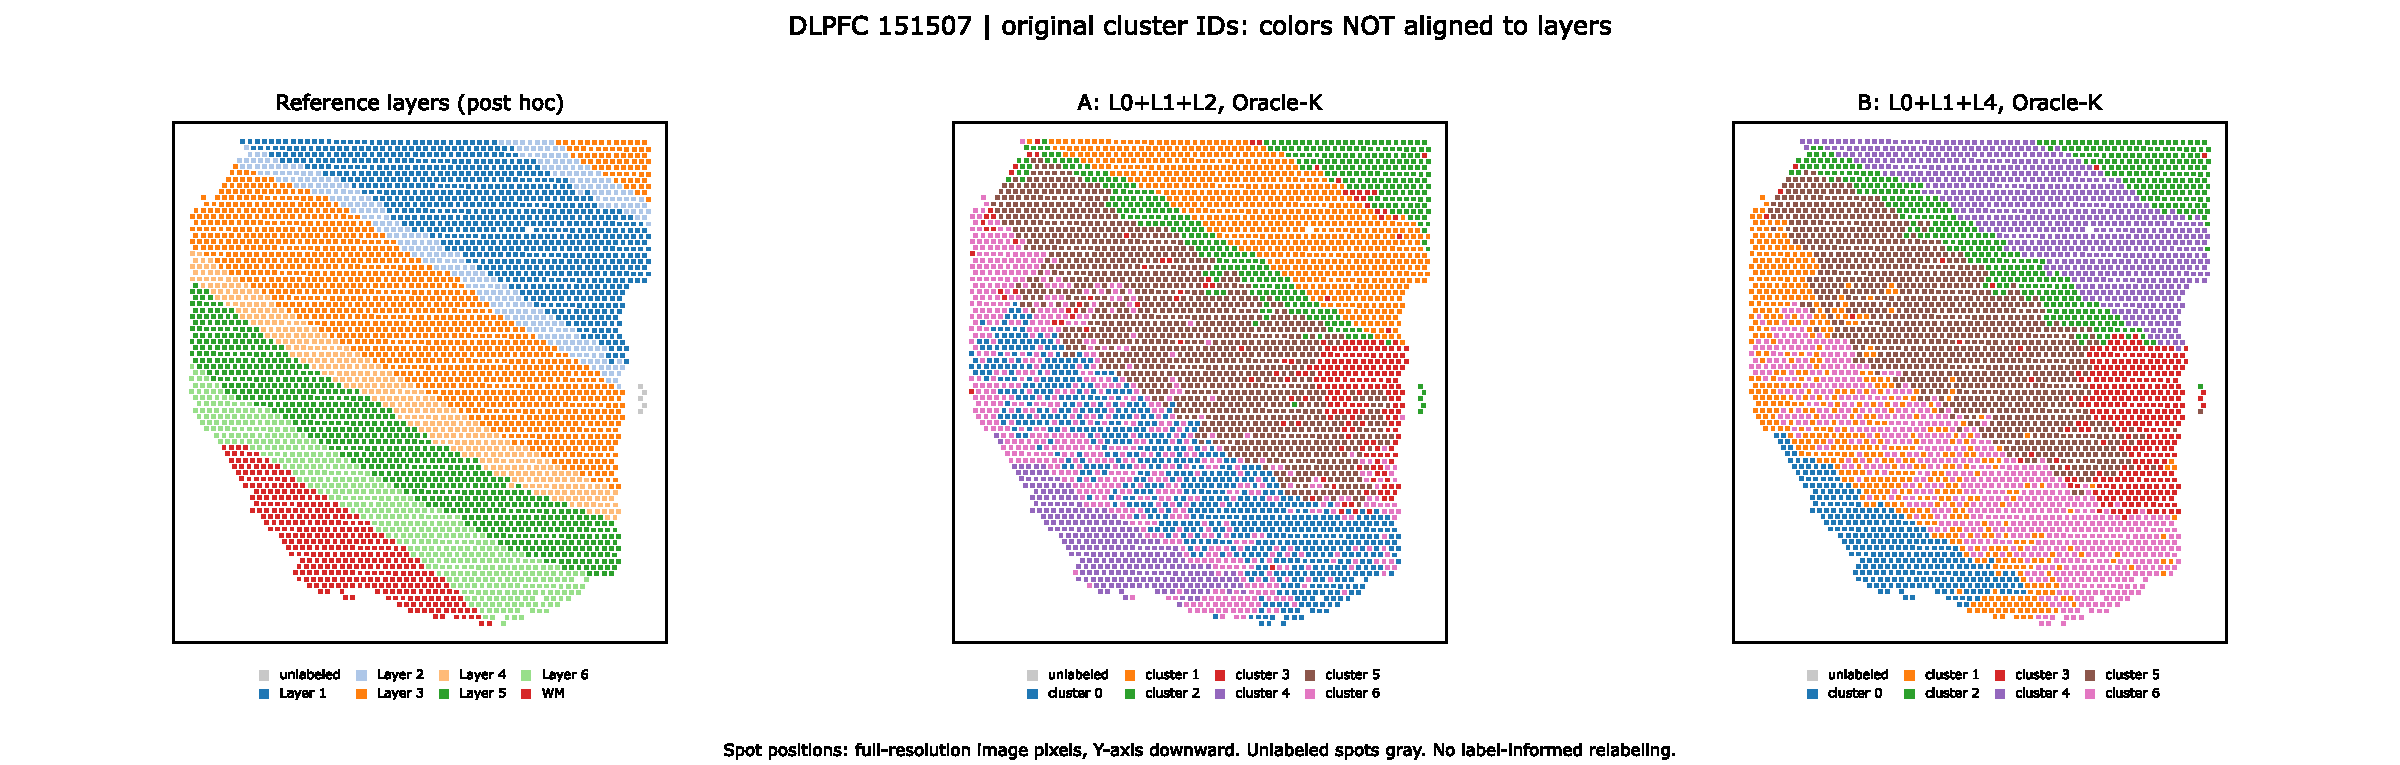
\includegraphics[width=0.98\linewidth]{E4_SOURCE_FIGURES_20261122_RELEASE/figures_pdf/151507/151507_reference_A_B_spatial.pdf}
\caption{DLPFC切片151507的参考组织层及冻结A15D、B15D原始聚类结果（E4真实SVG）。该切片按第一供体的B--A平均ARI正向代表规则选取；颜色不代表经过标签监督对齐的簇。}
\label{fig:cc-e4-151507-v1}
\end{figure}
}{%
\par\noindent\emph{[待插入E4原件：151507参考层/A15D/B15D空间三联图；目前GitHub尚未验收此SVG。]}\par
}
\IfFileExists{E4_SOURCE_FIGURES_20261122_RELEASE/figures_pdf/151671/151671_reference_A_B_spatial.pdf}{%
\begin{figure}[htbp]
\centering
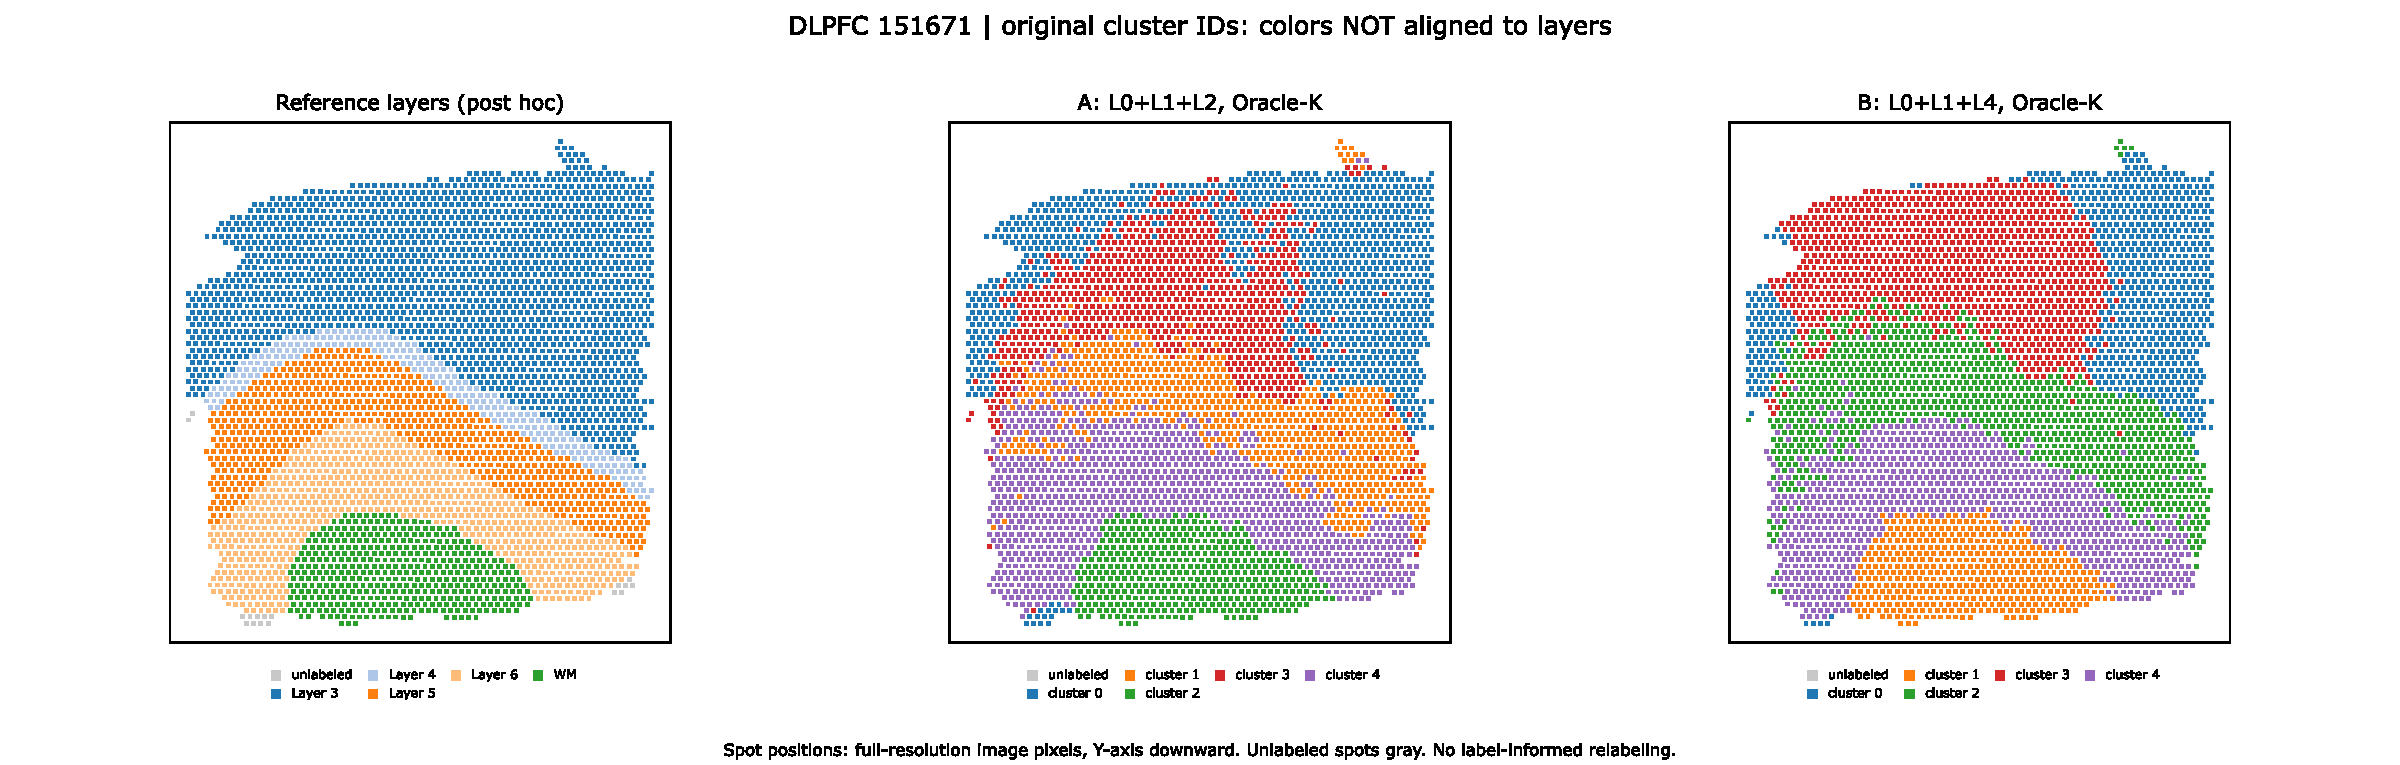
\includegraphics[width=0.98\linewidth]{E4_SOURCE_FIGURES_20261122_RELEASE/figures_pdf/151671/151671_reference_A_B_spatial.pdf}
\caption{DLPFC切片151671的参考组织层及冻结A15D、B15D原始聚类结果（E4真实SVG）。该切片按第二供体的B--A平均ARI接近零的规则选取。}
\label{fig:cc-e4-151671-v1}
\end{figure}
}{%
\par\noindent\emph{[待插入E4原件：151671参考层/A15D/B15D空间三联图。]}\par
}
\IfFileExists{E4_SOURCE_FIGURES_20261122_RELEASE/figures_pdf/151675/151675_reference_A_B_spatial.pdf}{%
\begin{figure}[htbp]
\centering
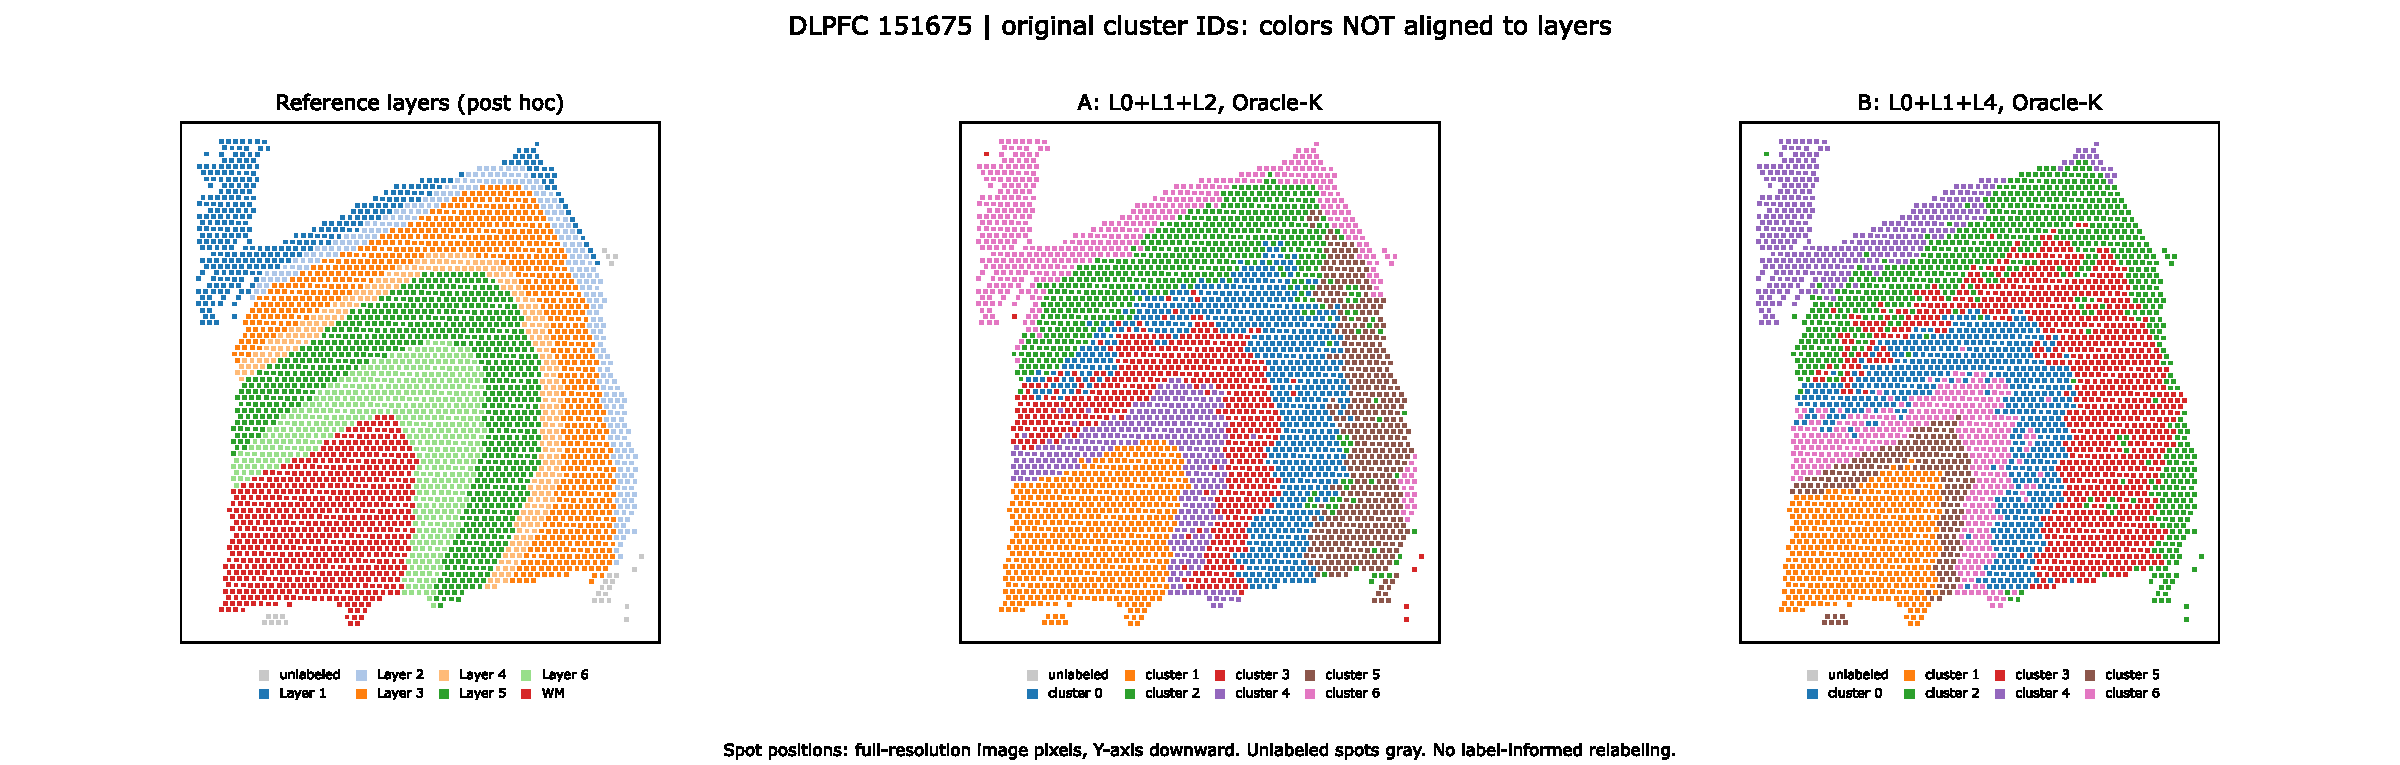
\includegraphics[width=0.98\linewidth]{E4_SOURCE_FIGURES_20261122_RELEASE/figures_pdf/151675/151675_reference_A_B_spatial.pdf}
\caption{DLPFC切片151675的参考组织层及冻结A15D、B15D原始聚类结果（E4真实SVG）。该切片按第三供体的B--A平均ARI负向代表规则选取。}
\label{fig:cc-e4-151675-v1}
\end{figure}
}{%
\par\noindent\emph{[待插入E4原件：151675参考层/A15D/B15D空间三联图。]}\par
}

为辅助理解皮层标记表达与空间域的关系，E4对每张切片的MOBP、PCP4、SNAP25三个标记基因分别从原始10x表达计数重新计算\texttt{log1p(10000$\times$基因UMI/spot总UMI)}，绘制统一颜色刻度范围0至6的表达图；对应原始与标准化数值保存在逐spot CSV。统一色标便于在图内比较表达分布，但图中的单个高表达区域不能直接作为人工组织层的独立验证，更不能证明某个聚类簇属于唯一确定的细胞类型。

\IfFileExists{E4_SOURCE_FIGURES_20261122_RELEASE/figures_pdf/151671/151671_MOBP_PCP4_SNAP25_expression.pdf}{%
\begin{figure}[htbp]
\centering
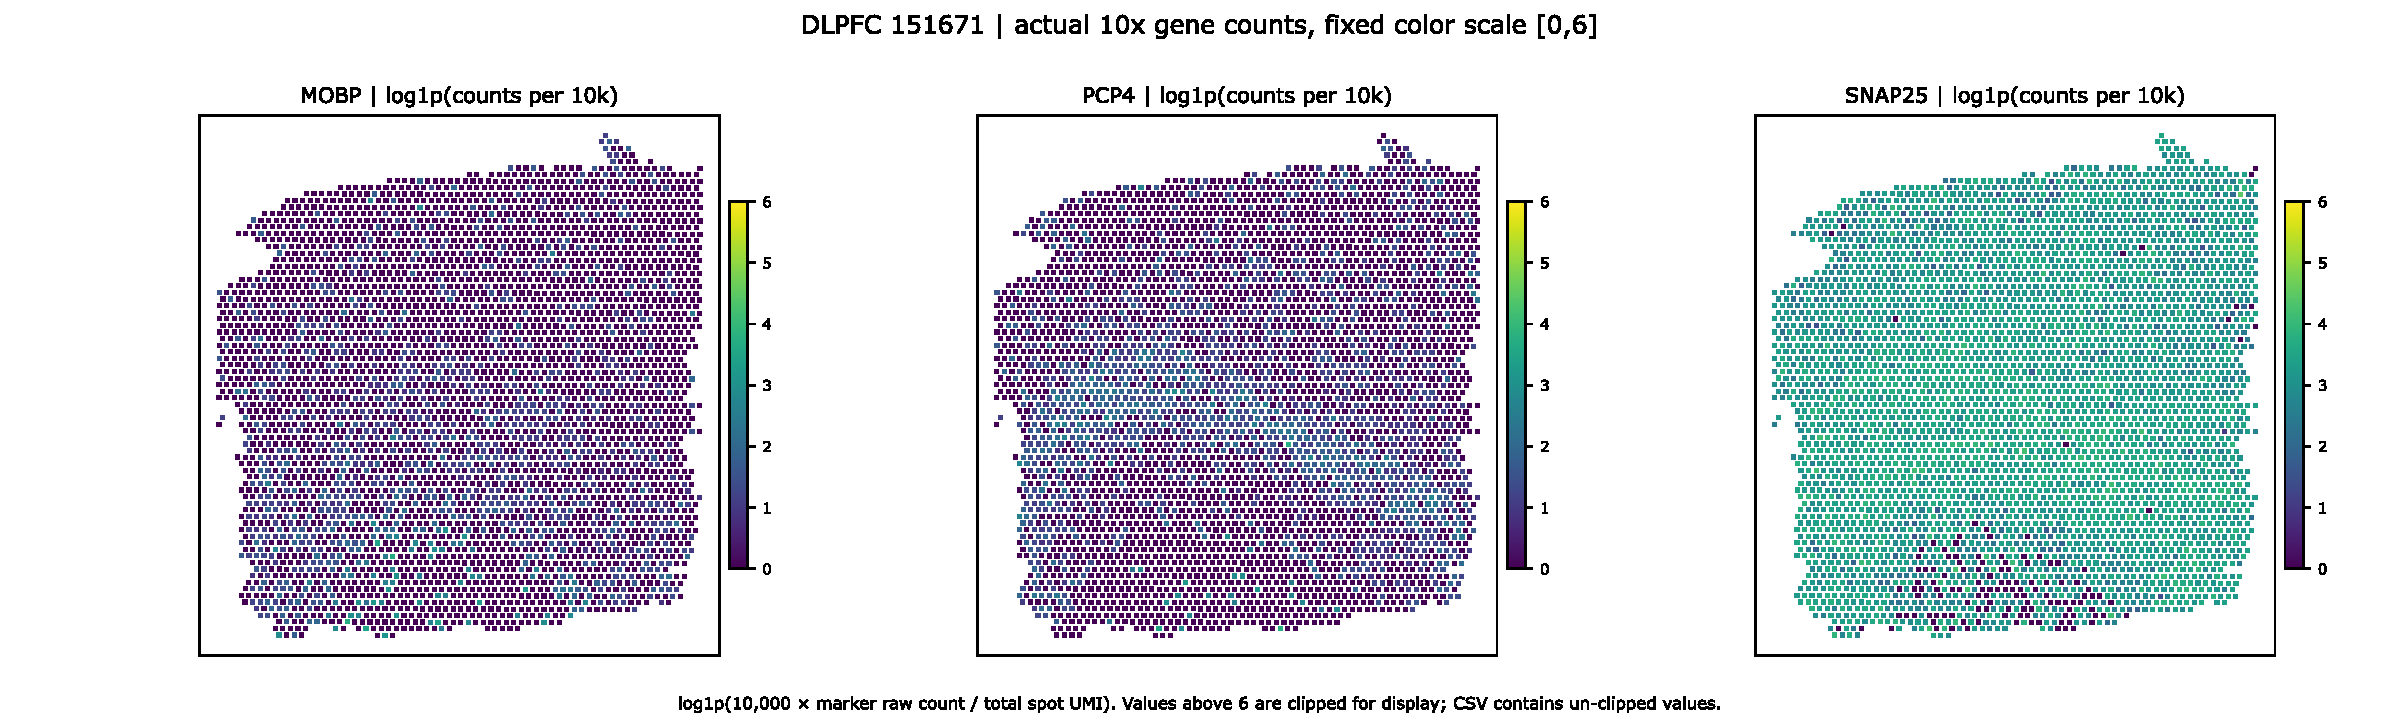
\includegraphics[width=0.98\linewidth]{E4_SOURCE_FIGURES_20261122_RELEASE/figures_pdf/151671/151671_MOBP_PCP4_SNAP25_expression.pdf}
\caption{DLPFC切片151671中MOBP、PCP4与SNAP25的原始计数归一化表达空间分布（E4真实SVG）。三图按相同归一化公式和0至6固定颜色范围展示。}
\label{fig:cc-e4-markers-151671-v1}
\end{figure}
}{%
\par\noindent\emph{[待插入E4原件：151671的MOBP、PCP4、SNAP25实际表达三联图。]}\par
}

此外，E4对每张切片分别生成参考组织层与A15D/B15D原始聚类编号的完整计数交叉表及可视化，保留未标注spot的排除数量。交叉表反映不同真实层对应的聚类标签构成，避免在无监督聚类编号之间强行建立没有证据的一一对应关系。原E4用户Windows独立审计报告12/12切片、36/36张SVG及36/36份CSV的产物完整性与输入SHA一致，并重新校核marker计数和交叉表；但\textbf{在这些源文件逐张上传GitHub并核对之前，本文不会新增对图上具体组织形态或局部marker模式的定量发现陈述}。

早期旧稿曾用151671与151676举例说明单种子下边界F1正负方向的差异；此处新E4图示固定的三张代表切片遵循另一套已记录的切片级\textbf{平均ARI}代表规则，不应将这两套事后案例选择依据混同。
 

\subsection{综合讨论及本章小结}
\label{subsec:cellcharter-discussion-v1}

本章的实证结果从三个互补维度说明，多尺度空间特征聚类的评价不能仅依据单一ARI均值。第一，在已冻结的Oracle-K与10技术种子条件下，累计邻域特征从5D扩展至25D时ARI和NMI的切片宏平均上升，但同维度的远邻块替换并未获得可重复的整体优势；尺度深度、特征维数和组织异质性共同影响比较结果。第二，无标签AutoK所得的簇数随切片和特征尺度改变，部分配置触及预定搜索边界；后验ARI/NMI显示尺度性能不是简单单调变化，因此固定K下较高的分数不能直接代替真实无标签应用场景的性能。第三，严格边界F1与1/2-hop容差F1呈现不同趋势，较深表征可能在容差允许的邻近边界检出上较高，却未改善精确边界位置。

成熟基线及外部队列进一步揭示结果的适用边界。A15D相对基础非空间设置在多个外部患者中出现方向一致的改善，但与BayesSpace的比较存在指标差异和明显的K-blind选K边界问题。6例乳腺癌患者中存在ARI接近零的低表现病例；这说明跨组织评价应保留患者级差异，而不能只给出一个全体宏平均值。上述结论支持把本项工作定位为\textbf{基于成熟CellCharter流程的多尺度与选K敏感性、空间边界定位及外部复核的系统实证评价}，而不是将已知特征聚合方法包装为新的基础算法。

本研究的限制主要包括：（1）DLPFC仅3名独立供体，且供体映射依据公开附录推定分组，仍需与原始元数据进一步核对；乳腺癌外部队列为6例患者，不宜作高精度群体推断；（2）部分原始实验使用标签类别数知情的Oracle-K，不能将其称为纯无监督选K表现；（3）不同空间方法的输入表征与计算路径并非完全相同，BayesSpace原冻结K-blind策略还存在频繁命中上界的缺陷；（4）邻域深度和输入维度共同变化，不能据此确定因果性空间平滑机制；（5）E3d后验评分与E3b容差属于观看既有结果后追加的分析，不能倒称前瞻注册的主终点；（6）用于展示的组织学标注具有数据集特定性，外部队列并非医学诊断金标准。

综上，在遵守数据来源、独立生物学单位和完整负结果报告的前提下，现有实验已经形成从固定尺度、K敏感性、严格与容差边界到成熟基线和外部组织数据的完整描述性证据链。后续论文章节应以真实实验记录、可复算结果和可核实文献说明研究贡献，不对尚未证明的算法创新或普遍性能优势作过度推断。
